% 2009 年江苏卷第 21A 题：四边形 ABCD，△ABC≌△BAD。
% 来源 PDF：普通高考/2009/2009江苏.pdf
% SHA-256：64e417d45911d88d77c047a419dcc259e7c7dc779c79d20df2092755c96a4501
% 原页：2009江苏.pdf 第 2 页（A3 三栏）第 2 栏，书页码 532。
% 绘制依据：按原页画四边形 ABCD（A 左下、B 右下、D 左上、C 右上）及对角线 AC、BD。
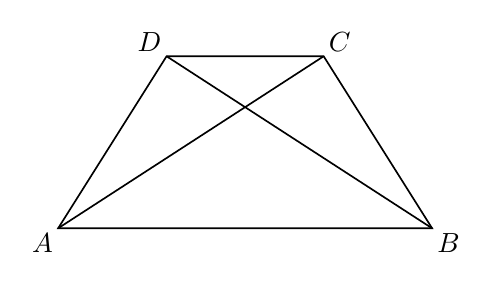
\begin{tikzpicture}[scale=0.95, semithick, every node/.style={inner sep=1.6pt}]
  \coordinate (A) at (0,0);
  \coordinate (B) at (5,0);
  \coordinate (C) at (3.55,2.3);
  \coordinate (D) at (1.45,2.3);

  \draw (A) -- (B) -- (C) -- (D) -- cycle;
  \draw (A) -- (C);
  \draw (B) -- (D);

  \node[below left] at (A) {$A$};
  \node[below right] at (B) {$B$};
  \node[above right] at (C) {$C$};
  \node[above left] at (D) {$D$};
\end{tikzpicture}
